\section*{\hypertarget{talent}{Talentos}}
\addcontentsline{toc}{subsection}{Talentos}%
"¡Santo cielo! ¡Una tortuga que habla!" \\
\indent - Bartz
\begin{center} 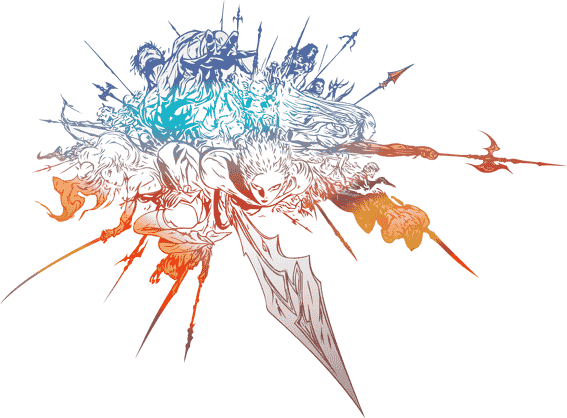
\includegraphics[width=1\columnwidth]{./art/images/ff14.png} \end{center}
%
Los talentos son habilidades que el personaje tiene y que no están relacionadas con el combate. Cada personaje empieza el juego con un talento y adquiere un segundo talento en el \textbf{Nivel 6}, adquirido a través de sus nuevas experiencias. El DJ también puede permitir que los personajes obtengan talentos adicionales en circunstancias especiales. A continuación, se muestran algunos Talentos que se pueden utilizar como se dan, pero el DJ también puede permitir que los jugadores creen sus propios Talentos utilizando los que ya existen como ejemplo. \\

\begin{description}[leftmargin=*]

\feat{Acampar de nuevo}
{
	Mientras estés en las afueras, puedes pasar una hora para crear un refugio cómodo para pasar la noche con los materiales que se encuentran en la naturaleza.
} 

\feat{Allévoy}
{
	Puedes imitar perfectamente el comportamiento y las expresiones de una persona con la que has pasado unos días.
}
	
\feat{Alquimista}
{
 Después de cada batalla exitosa contra monstruos, puedes dedicar unos minutos a crear un \hyperlink{item}{Fragmento de Bomb}, un \hyperlink{item}{Viento Ártico} o una \hyperlink{item}{Gema Eléctrica} utilizando sus restos. 
}

\feat{Apostador}
{
	Tienes \hyperlink{check}{Ventaja} en todas las tiradas relacionadas a juegos de azar, como las apuestas con dados o elegir una carta.
}

\feat{Aprendiz de Cid}
{
	Dados el tiempo y los materiales suficientes, puede reparar cualquier dispositivo o aparato roto. 
}

\feat{Asistente de Hope} 
{
	Puedes determinar la fecha y lugar de creación de cualquier objeto o rastro de manera precisa.
}

\feat{Artista del Tantalus}
{
	Puedes usar magia para crear efectos sencillos, como voces y sonidos, pequeñas llamas y ráfagas de viento.
}

\pagebreak

\feat{Bardo Holgazán}
{
	Has dominado perfectamente el instrumento musical que elijas. Además, puedes interpretar aceptablemente cualquier pieza musical en cualquier instrumento musical.
}


\feat{Calculador}
{
	Dado el tiempo suficiente, puedes resolver cualquier problema matemático. Además, puedes realizar estimaciones numéricas confiables (por ejemplo, calcular distancias o la cantidad de personas en un grupo).
}

\feat{Cantante de Repuesto}
{
	Tienes \hyperlink{check}{Ventaja} en todas las tiradas que impliquen actuar, cantar, bailar o interpretar en general.
}

\feat{Carpintero}
{
	Dados el tiempo y los materiales suficientes, puedes crear y reparar cualquier objeto que esté hecho principalmente de madera, incluyendo esculturas, muebles y vehículos.
}

\feat{Cauto como un Ladrón}
{
	Tienes \hyperlink{check}{Ventaja} en todas las tiradas relacionadas con la observación de posibles emboscadas u otras acciones hostiles de los personajes.
}

\feat{Cazador de Archylte}
{
 Tienes \hyperlink{check}{Ventaja} en todas las tiradas relacionadas con atrapar animales, incluyendo cazar y pescar.
}

\feat{Chef Curioso}
{
	Puedes pasar una hora preparando una comida sabrosa con casi cualquier cosa que puedas encontrar en tiendas o en la naturaleza.
}

\feat{Conductor designado}
{
	Puedes conducir o pilotear cualquier vehículo a la perfección, incluidos barcos y aeronaves. 
}

\feat{Conjurador}
{
	Puedes dedicar unos minutos para llevar a cabo un ritual que cree una ilusión de un personaje o monstruo, o un objeto de tamaño similar. Para entender que es una ilusión, un personaje tiene que tocarla o pasar una tirada con DC 8.
}

\feat{Discípulo de Llymlaen}
{
	Nunca pierdes el camino, incluso en lugares con los que no estás familiarizado. Además, no tienes problemas al leer mapas ni seguir direcciones dadas. 
}

\feat{Enemigo de Doma}
{
	Puedes pasar una hora para crear un potente veneno utilizando ingredientes que encuentres en la naturaleza o en tiendas. El veneno es líquido, sin sabor y sin olor, por lo que solo puede ser detectado por expertos como tú. Un personaje que consume el veneno hace una tirada con DC 8 y sufre \hyperlink{status}{KO} si falla. De lo contrario, pasa a estar \hyperlink{status}{Envenenado} por 3 turnos. 
}

\feat{Escáner}
{
	Cuando no estés en combate, puedes observar a un personaje para conocer inmediatamente su Nivel y su Oficio. También puedes realizar una tirada con DC 8 y, si tienes éxito, también conocerás sus talentos.
}

\pagebreak

\feat{Escéptico}
{
	Tienes \hyperlink{check}{Ventaja} en todas las tiradas relacionadas con discernir si alguien está mintiendo o reteniendo información.
}

\feat{Escudo del Rey}
{
	Tienes \hyperlink{check}{Ventaja} en todas las tiradas que dependan principalmente de la fuerza, como levantar los objetos pesados o abrir tapas de recipientes muy ajustadas.
}

\feat{Excalipoor}
{
	Siempre que veas una pieza de equipo, puedes comprender de inmediato sus efectos especiales. Además, cada vez que mejores armas y armaduras para tu uso personal, solo te cuesta la mitad del Gil habitual.
}

\feat{Farmacólogo}
{
	Cada vez que utilices un \hyperlink{item}{Objeto} fuera de combate sobre ti mismo, obtienes los siguientes beneficios adicionales: si el artículo aumenta tus PV, recuperas el doble de lo habitual. De lo contrario, recupera 1d PV además de su efecto habitual. 
}

\feat{Florista} 
{
	Puedes identificar cualquier planta y saber cómo hacerla crecer incluso en situaciones muy desfavorables.
}

\feat{Geomante}
{
	Tienes \hyperlink{check}{Ventaja} en todas las tiradas que requieran competencia y experiencia relacionadas con la naturaleza, como seguir un rastro en un bosque. 
}

\feat{Guardia} 
{
	No sufres ningún daño si caes desde cualquier altura.
}

\feat{Guía}
{
	Tienes \hyperlink{check}{Ventaja} en todas las tiradas relacionadas con encontrar ubicaciones y pasajes ocultos. 
}

\feat{Historiador de Spira}
{
	Tienes conocimiento sobre todos los hechos históricos importantes de todo el mundo. Además, tienes \hyperlink{check}{Ventaja} para recolectar información histórica y hacer conexiones con los eventos históricos más oscuros. 
}

\feat{Jugador Estrella}
{
	Eres uno de los mejores del mundo en un deporte o juego que elijas.
}

\feat{La Fortuna Me Sonríe}
{
	Cada vez que obtengas un resultado total de 2 en una tirada fuera de combate, puedes volver a hacer la tirada.
}

\feat{Líder}
{
	Tienes \hyperlink{check}{Ventaja} en todas las tiradas que implican impresionar o persuadir a alguien a través del habla. 
}

\feat{Mago Azul}
{
 Puedes aprender rápidamente habilidades simples que no sean de combate observando cuidadosamente a alguien competente durante un tiempo. Estas habilidades simples son, por ejemplo, cocinar una comida o montar un \hyperlink{chocobo}{Chocobo}.
}

\pagebreak

\feat{Meteorólogo}
{
	Puedes predecir con precisión el clima de tu ubicación actual durante la próxima semana.
}

\feat{Mognet}
{
	Puedes enviar mensajes telepáticos a cualquier persona que puedas ver. Si el destinatario está a más de 100 u de ti, debe pasar primero una tirada con DC 7.
}

\feat{¿No Nos Conocemos?}
{
	Siempre que te encuentres con un personaje nuevo, puede declarar que lo has conocido antes. Si lo haces, el DJ decide qué tipo de conexión tienes con ese personaje. Solo puedes utilizar este efecto un total de 3 veces en toda la aventura.
}

\feat{O’aka XXIV}
{
	Siempre que vendas bienes a alguien que esté dispuesto a comprarlos, puedes convencerlo de que te los compre a su valor original a pesar de ser usados.
}

\feat{Oculto} 
{
	Tienes \hyperlink{check}{Ventaja} en todas las tiradas relacionadas con ocultarte o evitar ser detectado.
}

\feat{Ojo Talentoso}
{
	Puedes capturar imágenes perfectas de escenas, paisajes y personas en una pintura o fotografía. 
} 

\feat{Orador}
{
	Siempre que hables con un personaje que conozcas, puedes dedicar unos minutos a motivarlos e inspirarlos. El personaje tiene \hyperlink{check}{Ventaja} en la siguiente tirada que realice.
}

\feat{Políglota}
{
	Manejas con fluidez dos idiomas y puedes aprender otros en cuestión de días.
}

\feat{Químico}
{
 Puedes pasar una hora para crear una \hyperlink{item}{Poción} o un \hyperlink{item}{Remedio} utilizando ingredientes que encuentres en la naturaleza o en tiendas.
}

\feat{Sabio de los Chocobo}
{
 Puedes domar y construir amistades con animales y monstruos amigables como los \hyperlink{chocobo}{Chocobos}.
}

\feat{Teólogo}
{
 Tienes un vasto conocimiento sobre todas las religiones del mundo, incluyendo sus deidades, así como sus diferentes costumbres y divisiones.
}

\feat{Tejedor}
{
 Dados el tiempo y los materiales suficientes, puedes crear cualquier tipo de tejido o ropa.
}

\feat{Yin y Yang}
{
 Cuando no estés en combate, puedes meditar durante unos minutos para obtener el siguiente beneficio: reduces tus PM por la cantidad que elijas y aumentas tus PV por la misma cantidad.
}

\end{description}

\pagebreak